\section{Simulation}
In this chapter, we empirically test the performance of our proposed and the already existing estimators for \ac{SC} in different \ac{DGP}. Independent of the specific features of the data in terms of pre- and post-treatment period length and the prevailing time series structures, we proceed as follows: We simulate $T_{pre} = T_0 -1$ periods of pre-treatment and $T_{post} = T - (T_0 -1)$ periods of post-treatment data for the single treated unit and the $J$ donor units. Each estimator's main goal is to grasp the consistent patterns before treatment and accurately extend these patterns into the time after treatment. Said differently, the pre-treatment phase depicts the training set of the models and the post-treatment the validation set. To root the simulation framework as close as possible to real-world \ac{SC} applications, we define $T_{pre}$ and $T_{post}$ such that their range is comparable to low-frequency macroeconomic settings, i.e. $T_{pre} \in \left\lbrace 20,50,100\right\rbrace $ and $T_{post} \in \left\lbrace 10,20,30\right\rbrace$. Furthermore, we consider two types of \ac{DGP}, a static factor process and a dynamic \ac{VAR}-process that is inspired by real \ac{GDP} processes of the G20 countries.

\subsection{Static Data Generating Processes}

In their \ac{SC} application of estimating the causal effect of California's proposition 99, \cite{abadie:2010} suppose that the (potential) outcome $Y_{i,t}^{N}$ follows a factor model of the  form 
\begin{equation*}
	Y_{i,t}^{N} = \alpha_t + \theta_t Z_i + \lambda_t \mu_i + \epsilon_{it}.
\end{equation*}
$\alpha_t$ denotes an unknown panel-invariant factor, $Z_i$ is a vector of observed panel-specific covariates, $\theta_t$ is a vector of unknown parameters, $\lambda_t$ is a vector of unknown common factors and $\mu_i$ are panel-specific unknown factor loadings. The unobserved shocks $\epsilon_{it}$ have zero mean at the panel level. 
For this specific setting, \cite{abadie:2010} show that "[...] the bias of the SC-estimator can be bounded by a function that goes to zero as the number of pre-treatment periods increases." Further the number of donor units has to be fixed. The fact, that $\alpha_t$ is panel-invariant seems minor at first glance. However, as the \ac{SC}-estimator does neither contain an intercept nor does it allow for extrapolation outside the convex hull of the donor pool, the unbiasedness of the estimator directly depends on the distribution of the intercepts. In a slightly more realistic data-generating scenario, the intercepts do not follow a degenerate point distribution with $P(X = 0) = 1$ but are drawn from a symmetric distribution centered around the origin like the standard normal. 

\cite{ferman:2021} considers a de-meaned scenario without additional covariates. In our simulation, we follow the basic set-up of Ferman and generate data according to a similar factor model. However, we consider it more realistic to add a time-invariant and panel-specific intercept to the (potential) outcome instead of analyzing a de-meanded \ac{DGP}. Our representation of the counterfactuals therefore boils down to 
\begin{equation*}
	Y_{i,t}^{N} = \alpha_i + \lambda_t \mu_i + \epsilon_{it}.
\end{equation*}
In this simplified setting, the counterfactual is given by the composition of the unknown panel-specific factor loadings $\mu_i$ and the $F$ unknown common factors $\lambda_t = (\lambda_{1,t}, ..., \lambda_{F,t})$ plus intercept $\alpha_i$ and idiosyncratic shocks $\epsilon_{it}$. For the sake of simplicity, Ferman considers a scenario with only two common factors, $\lambda_{1,t}$ and $\lambda_{2,t}$. We proceed analogously and generates the data such that the (potential) outcome of the treated unit and the first half of the donor pool load exclusively with loading one on the first factor, the remaining donors load exclusively with loading one on the second factor. Therefore $\mu_i$ is a $(2 \times 1)$-column-vector with the first (second) entry being one and the second (first) entry being zero for the first (second) half of the donor pool. Further, the random variables $\alpha_i, \lambda_{1,t}, \lambda_{2,t}$ and $\epsilon_{it}$ are realizations of \ac{iid} standard normal distributions $\mathcal{N}(0,1)$. The following figure exemplifies the functionality of the \ac{DGP} with $T_{pre} = 20$ and $T_{post} = 10$ and a constant treatment effect of $\delta_{1,t} = 10$ for $t > T_0$.\footnote{In this example, the series $j = 0$ is treated at $T_0 = 20$, while the impact of the treatment becomes noticeable one time period later, starting from $t > T_0$. Note that the actual treatment effect is irrelevant for our investigation as it is empirically observable.}  
\begin{figure}[H]
	\centering
	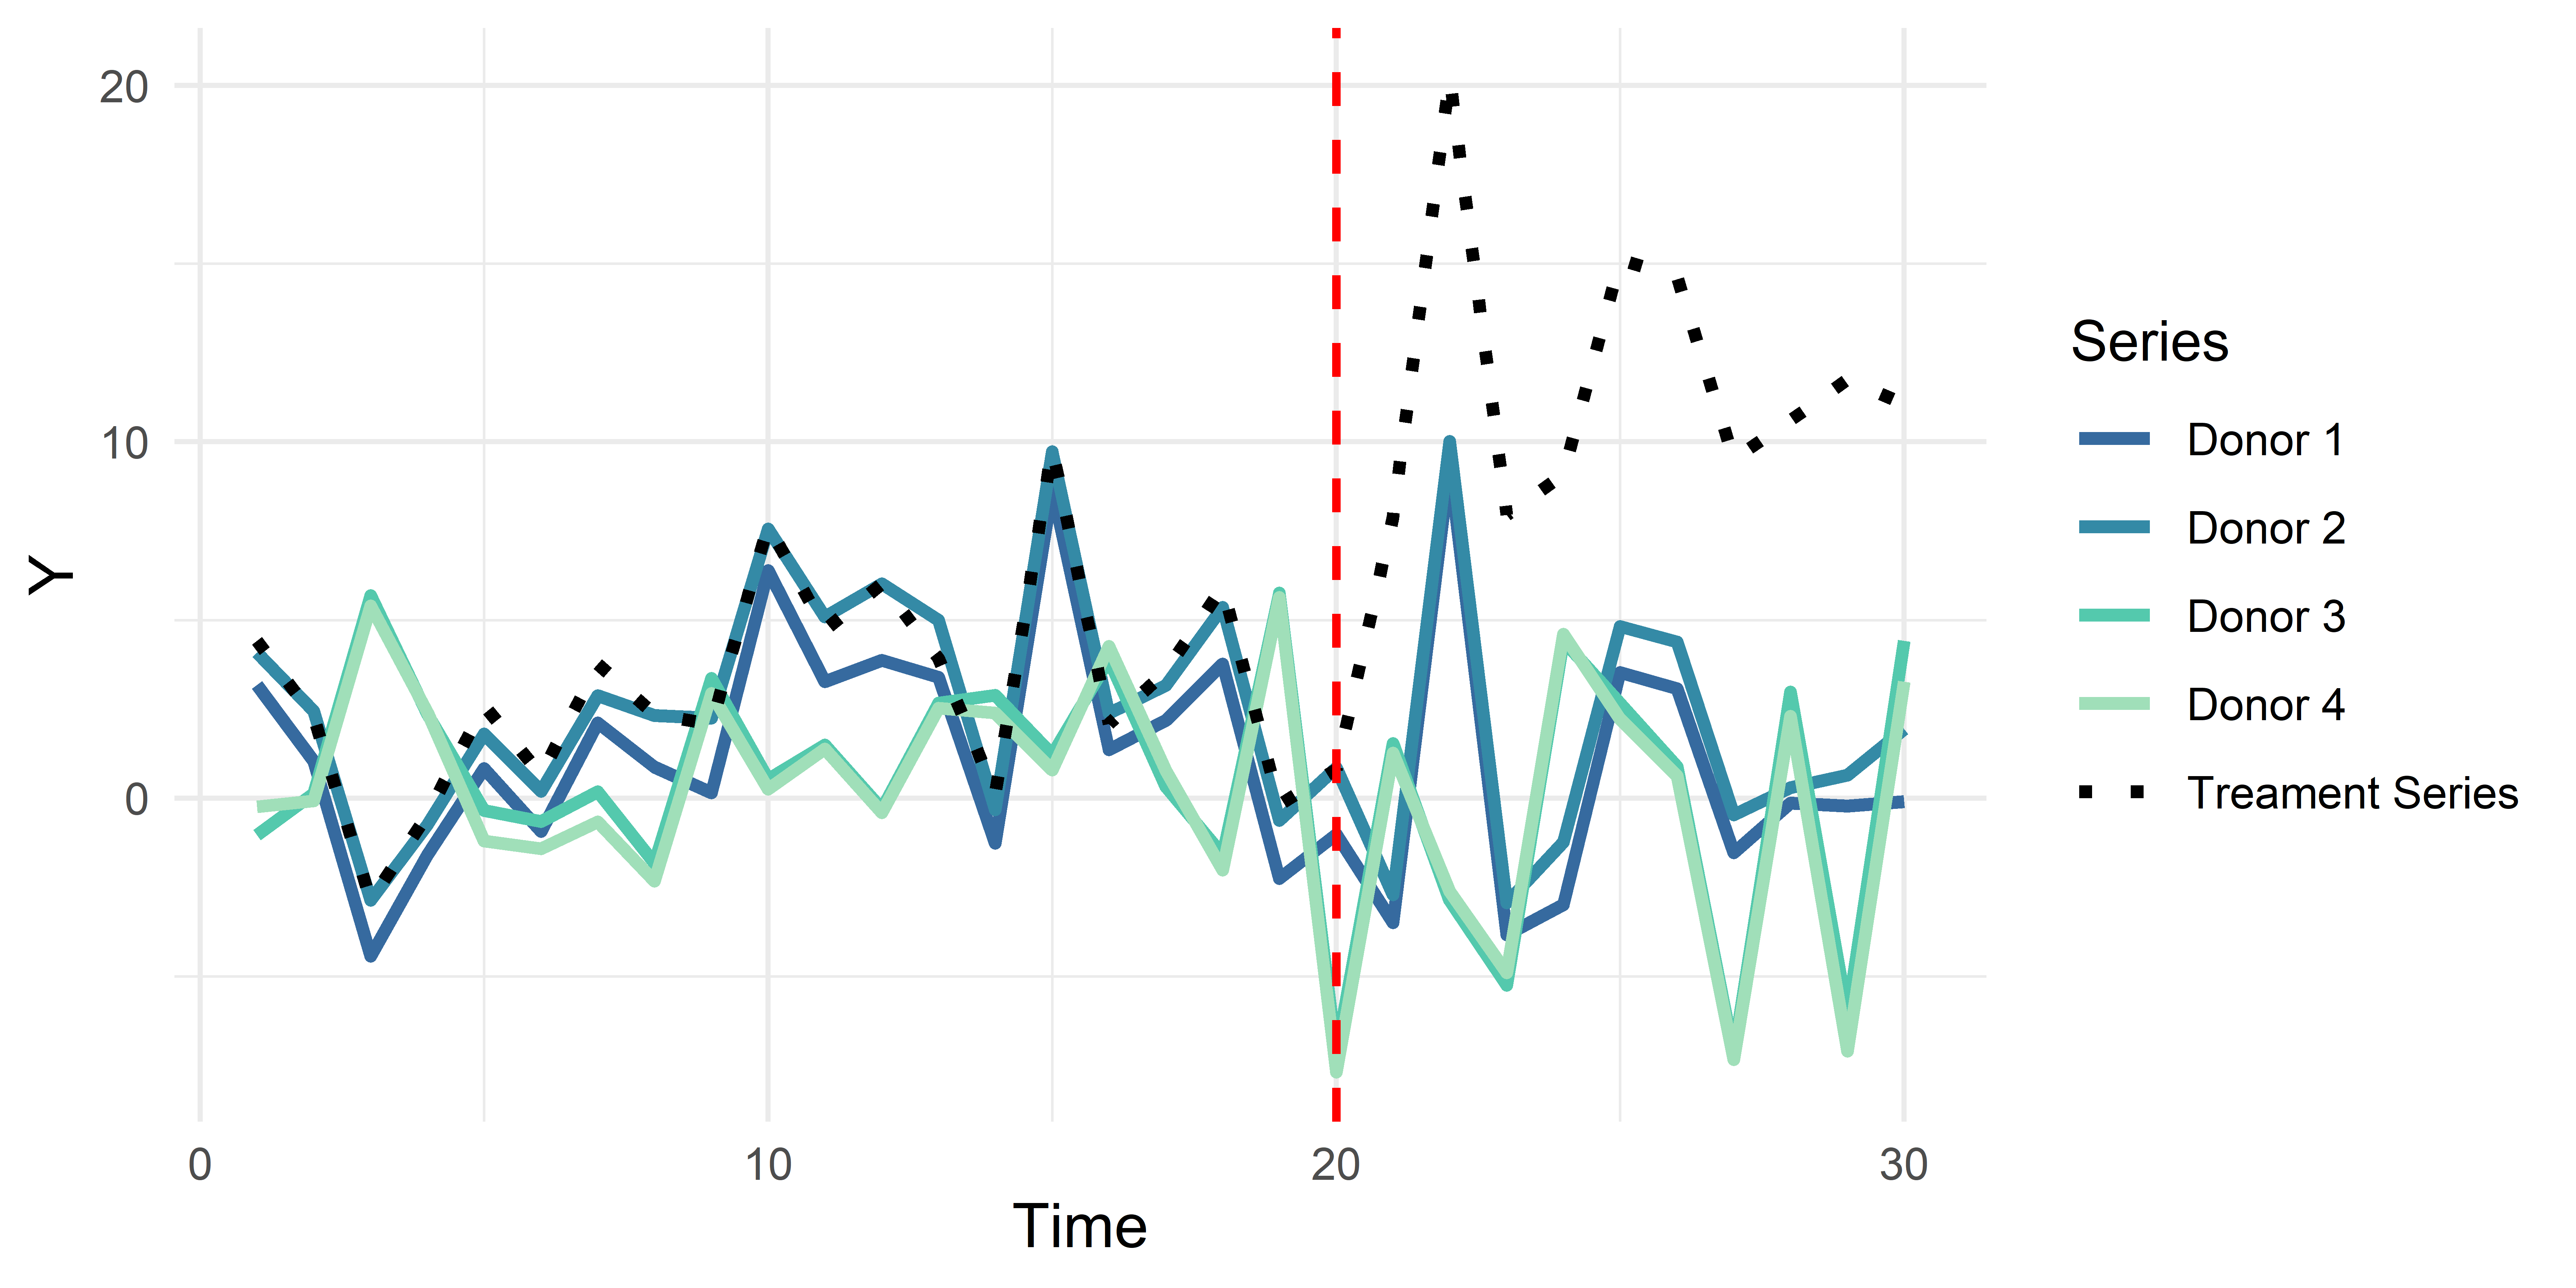
\includegraphics[scale=.9]{F02}
	\caption{Example Factor-\ac{DGP}}
	\label{F_02}
\end{figure}
To make the factor structure easy to see, we scaled the factor variance by $10^1$ and the error variance by $10^{-1}$. The generated data exhibits a clearly observable factor structure: The treatment unit and the first half of the donors (Donor 1 and 2) as well as the second half of the donors (Donor 3 and 4) share a common factor. Thus, the objective of each employed method is to recover the true factor structure, i. e. irrelevant of the size of donor pool to weight only the first $\frac{J}{2}$ donors positively. Further, we see that each series possesses an own intercept. Yet, the intercept variation is dominated by the factor variation as in this example \ac{DGP} only, there variance has been scaled by 10.

\textit{EMPLOYED MODELS} \\
For the static factor \ac{DGP}, we consider five models: 
\begin{enumerate}
	\item SC: The first model is the ordinary \ac{SC} method without additional covariates. Therefore, this method is equivalent to a restricted \ac{OLS} regression that regresses the treatment series on the donors series given the constraint of no intercept and non-negative coefficients that sum up to one. The belief for this model is that the untuneable restrictions prevent it from overfitting the pre-treatment data but that this inelasticity comes at the costs of a reduced predictive performance.
	\item OLS: The second model is a usual regression that regresses the treatment series on the donor series. The belief for this model is that it starts overfitting the pre-treatment data as $J$ grows large. Further for $J > T_0$, it is unable to provide any prediction or forecast.
	\item NET: The third model we consider is the aforementioned mentioned elastic net as proposed by \cite{doudchenko:2016} in the context of \ac{SC}. Due to its flexible hyperparameters tuned via pre-treatment cross-validation, we expect this model to perform reasonable well both before and after the treatment. In the conceptual introduction of the elastic net, we stressed the potential drawback of having no closed form solution. As a consequence, we assume the model to perform worse in small samples.
	\item REGSC: The fourth model under consideration is our proposed regularized synthetic control model which can be interpreted as a mixture of the elastic net and the original \ac{SC} estimator. It is comparable to the elastic net insofar that it simply substitutes the Lasso-shrinkage by the inverse-Ridge-shrinkage. This regularization is motivated by the \ac{SC} specificity of having percent-like coefficients. Thus, we expect the model to perform well especially in settings that are comparable to the original \ac{SC} setting like the static factor \ac{DGP}. Its closed form solution and the increased flexibility caused by the tuneable hyperparameters make us confident that the model performs equally well in small and in large as well as in the pre- and the post-treatment period.		   
	\item FACTOR: The data of this chapter is generated such that the common factors and the idiosyncratic component are uncorrelated and that the idiosyncratic errors are mutually uncorrelated. Thus, the static factor model which estimates the common factors as linear function of the donors is the most natural candidate model.  A popular estimator for the factor model is the \ac{PC} estimator. In the pre-treatment period, we obtain the predictions by regressing the treatment series on the "latent" factors. As we implemented a two-factor structure, the factors are computed by multiplying the first two eigenvalues of the covariates matrix with the matrix of the covariates. The forecasts for the post-treatment period are obtained by multiplying the factor structure of the post-treatment period with the regression coefficients of the pre-treatment regression. As this model directly build upon the \ac{DGP}, it is our "benchmark-model" and we expect it to perform best among all candidates. 
	\textcolor{magenta}{\textbf{(why no overfitting?)}} 
\end{enumerate}
\textcolor{magenta}{\textbf{(what else?)}} 



\begin{itemize}
	\item All simulations are conducted with 1,000 iterations per combination of pre- and post-treatment horizon and donor quantity. \textcolor{magenta}{\textbf{(Important to distinguish different intercept cases: If the intercept of the treated series falls outside the donor-intercepts, SC exhibits a bias as it does not allow for a panel-specific constant.)}} 
	\item employ RMSE as loss function. Quadratic loss, tremendously important in practice. Reasonable approximation to realistic loss structures and mathematically convenient (\cite{diebold:2017})
\end{itemize}

%\item \cite{abadie:2010} suppose that the counterfactuals $Y_{1,t}^{N}$ for $t > T_0$ are given by a factor model of the form $Y_{i,t}^{N} = \alpha_t + \theta_t Z_i + \lambda_t \mu_i + \epsilon_{it}$. $\alpha_t$ denotes an unknown common factor with constant loadings across panel units. $Z_i$ is a vector of observed panel-specific covariates, $\theta_t$ is a vector of unknown parameters, $\lambda_t$ is a vector of unknown common facots and $\mu_i$ are panel-specific unknown factor loadings. The unobserved transitory shocks $\epsilon_{it}$ have zero mean at the panel level. For this specific setting, \cite{abadie:2010} show that "[...] the bias of the SC-estimator can be bounded by a function that goes to zero as the number of pre-treatment periods increases." Further the number of donor units has to be fixed.

%\item \cite{ferman:2021} considers a de-meaned scenario without additional covariates. The representation of the counterfactuals therefore boils down to $Y_{i,t}^{N} = \lambda_t \mu_i + \epsilon_{it}$. Thus the counterfactual is given by the composition of the unknown panel-specific factor loadings and the unknown common factors plus the idiosyncratic shocks.

%\item We re-estimated the Tobacco Control and the Basque application and found that the inclusion of additional covariates did not improve the predictive accuracy of the SC estimator. Therefore, we follow the simulation suggestion of \cite{ferman:2021} and root our simulation in his proposed factor model without additional covariates. 

%\item Analogous to Ferman, we consider a setting with two common factors, $\lambda_{1,t}$ and $\lambda_{2,t}$. The potential outcomes for the treated unit and for the first half of the donor pool load exclusively with loading one on the first factor, the remaining donors load exclusively with loading one on the second factor. Therefore $\mu_i$ is a $(2 \times 1)$-rowvector with the first (second) entry being one and the second (first) entry being zero for the first (second) half of the donor pool.	

%\item In each simulation, we simulate a total of $T_0 + T_1$ observations, where $T_0$ represents the length of the pre- and $T_1$ the length of the post-treatment period. In order to have a simulation framework that is as close as possible to real world SC-applications, we choose $T_0 \in \left\lbrace 20,50,100\right\rbrace $ and $T_1 \in \left\lbrace 10,20,30\right\rbrace $. Further, we define the size of the donor pool as $J \in \left\lbrace 5,10,15,20,25,30\right\rbrace$.

%\item To initialize the simulation, we simulate the two common factors by drawing $T_0 + T_1$ \ac{iid}  observations from a standard normal distribution. Next, we multiply the common factors for all donors and the treatmend unit with the factor loadings $\mu_i$ and add \ac{iid} standard normal shocks. Additionally, we add panel-specific \ac{iid} standard normal intercepts such that our \ac{DGP} takes the following form: $Y_{i,t}^{N} = \gamma_i + \lambda_t \mu_i + \epsilon_{it}$. 

%\item Figure \ref{F_02} visualizes one potential \ac{DGP} with $T_0 = 20$ and $T_1 = 10$. To make the factor structure visible, we scaled the factor variance by $10^1$ and the shock variance by $10^{-1}$. Moreover, for better eyeball inspection, we added a constant treatment effect of $\delta_{1,t} = 10$ for $t > T_0$. Note that the specific nature of the treatment effect is irrelevant for our investigation. Since $Y_{1,t}^T$ is observable for $T>T_0$, we can choose an arbitrary functional form or even implement no treatment effect at all. 

%\item The described factor structure is inherent in Figure \ref{F_02}: The treatment unit and the first half of the donors (Donor\_1 and Donor\_2) as well as the second half of the donors (Donor\_3 and Donor\_4) share a common factor structure. The constant treatment effect is added after $T_0 = 20$ periods, resulting in a 10 unit vertical shift of the treatment series.

%\item We consider five different models whose goal is to recover the true factor structure of the treatment unit in the pre-treatment period and to predict the counterfactual in the post-treatment period as accurately as possible. Put differently, we train the models on $T_0$ pre-treatment observations and test their performance using $T_1$ post-treatment observations.

%\item Synthetic-Control-Model (SC): In case of no additional explanatory variables, the \ac{SC}-approach reduces to a constraint regression that regresses the treatment series on the donor series given the constraint of no intercept and non-negative coefficients that sum up to one. \ac{ADH} argue that the constraints prevent the SC models from over-fitting, but they do so at the cost of a reduction in flexibility.
%\item Regularized OLS-Model (REGOLS): Our proposed model. We allow for a constant and arbitrary coefficient values. We propose a two-dimensional regularization: A ridge/l2-norm penalty that penalizes the coefficient sum and a second penalty term that shrinks the coefficient sum towards one. We identify the optimal hyperparameter-combination by applying a 50/50 train-test-split in the pre-treatment period on a two-step random grid search. In the first step, we randomly select 400 hyperparameter-combinations from a $(50 \times 50)$-grid. In the second step, we enclose the potential optimum by sequentially holding the first and the second hyperparameter fixed while increasing and decreasing the remaining hyperparameter on a coarser grid. 
%\item Elastic Net (NET): \cite{doudchenko:2016} propose to estimate the counterfactual using an elastic net regression. 
%\item OLS-Model (OLS): Finally, to verify the belief that a simple linear model overfits the training data and therefore yields poor forecasting accuracy in the testing period, we also employ an ordinary least squares model.


\subsection{Dynamic Data Generating Processes}